\documentclass{jhwhw}
\usepackage{adjustbox}
\lstset{
  basicstyle=\ttfamily\small, % Small font size for code
  breaklines=true,            % Enable line breaking
  postbreak=\mbox{\textcolor{red}{$\hookrightarrow$}\space}, % Optional: mark where the line was broken
}
\author{Deepak Nathani}
\title{CS292C Homework 2}
\begin{document}
\maketitle

\section{Self-Grade}

\begin{table}[h]
    \centering
    \begin{tabular}{l|c}
        \toprule
        \midrule
        \textbf{Problem} & \textbf{Self-Grade} \\
        \midrule
        {1: Problem Name 1} & {2} \\
        \midrule
        {2: Problem Name 2} & {2} \\
        \midrule
        {3: Problem Name 3} & {2} \\
        \midrule
        {4: Problem Name 4} & {2} \\
        \midrule
        {5: Problem Name 5} & {2} \\
        \midrule
        {6: Problem Name 6} & {2} \\
        \midrule
        {7: Problem Name 7} & {2} \\
        \midrule
        {8: Problem Name 8} & {2} \\
        \midrule
        {9: Problem Name 9} & {2} \\
        \midrule
        {10: Problem Name 10} & {1} \\
        \midrule
        {11: Problem Name 11} & {0} \\
        \midrule
        \bottomrule
    \end{tabular}
\end{table}

\section{Problems}
\problem{Install OCaml}
Install OCaml by following the instructions in \texttt{install.md}.
Once you're done, enter \texttt{utop} and evaluate the following expression:
\begin{lstlisting}
print_endline "I have installed OCaml!"
\end{lstlisting}
Include a screenshot of all of \texttt{utop}'s output thus far (including the welcome message) to your PDF file.
\newline
\solution
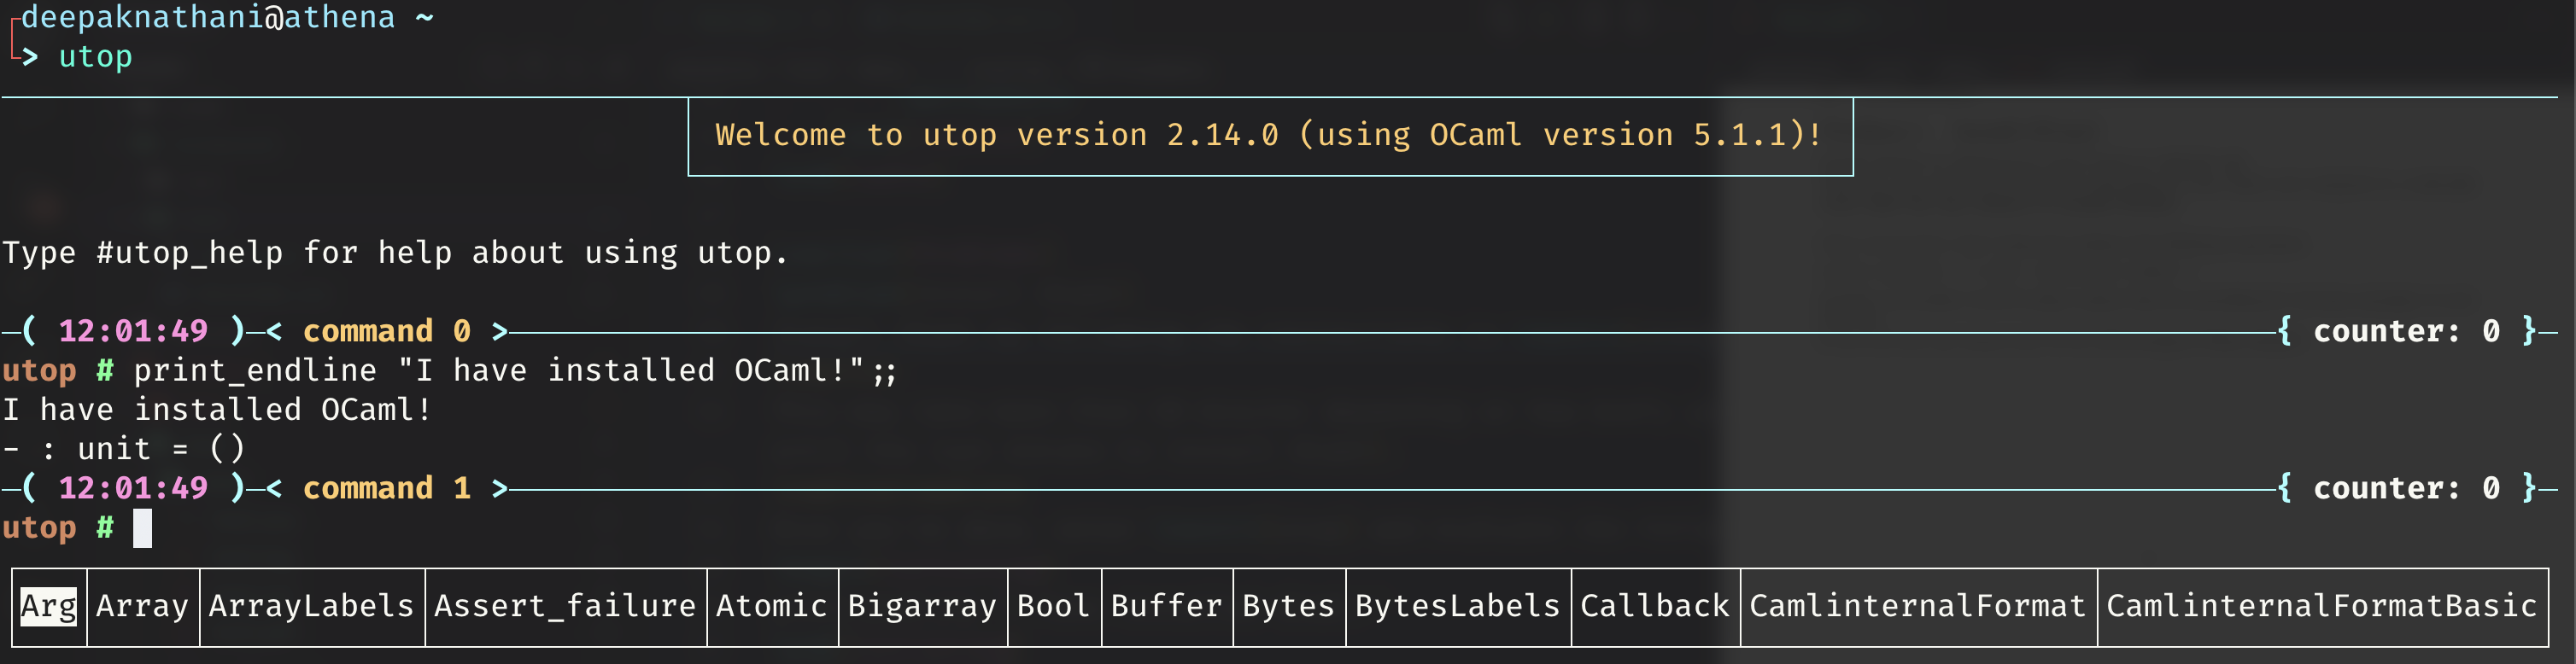
\includegraphics[width=\textwidth]{assets/problem1.png}

\problem{Compress/Duplicate Removal}
\solution
\part
\begin{lstlisting}
let rec compress (equal: 'a -> 'a -> bool) (l: 'a list) : 'a list = 
match l with
| [] -> []
| [x] -> [x]
| x::(y::_ as t) ->
    if equal x y then
    compress equal t 
    else
    x::(compress equal t)
\end{lstlisting}
\bigskip
\part
\begin{enumerate}
    \renewcommand{\labelenumi}{\arabic{enumi}.}
    \item \textbf{TestCase 1:} Empty string\newline
    \begin{lstlisting}
        let b = [] in compress String.equal b;;
    \end{lstlisting}
    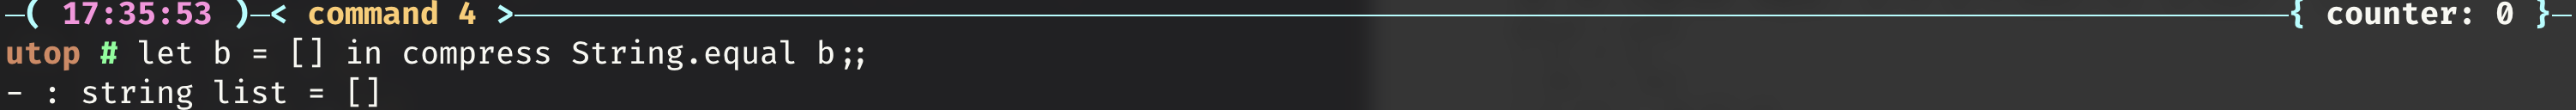
\includegraphics[width=\textwidth]{assets/q2tc1.png}
    \item \textbf{TestCase 2:} String list with both consecutive and non-consecutive repeating characters.\newline
    \begin{lstlisting}
        let b = ["a"; "a"; "b"; "b"; "a"; "a"] in compress String.equal b;;
    \end{lstlisting}
    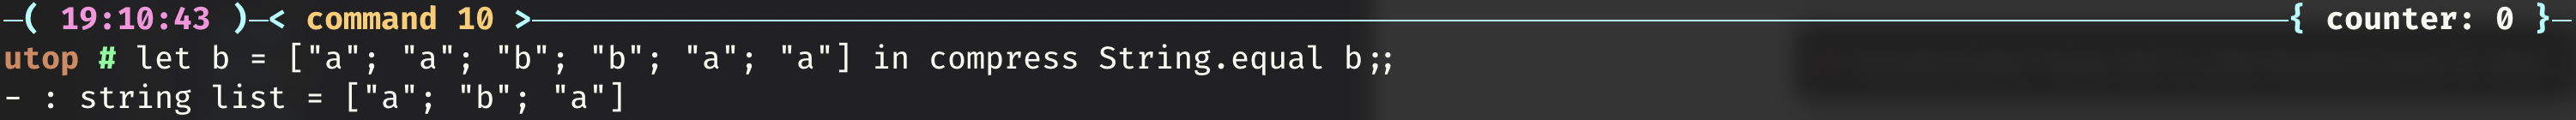
\includegraphics[width=\textwidth]{assets/q2tc2.png}
    \item \textbf{TestCase 3:} Int list with no repeting characters.\newline
    \begin{lstlisting}
        let b = [1; 2; 3; 4; 5] in compress Int.equal b;;
    \end{lstlisting}
    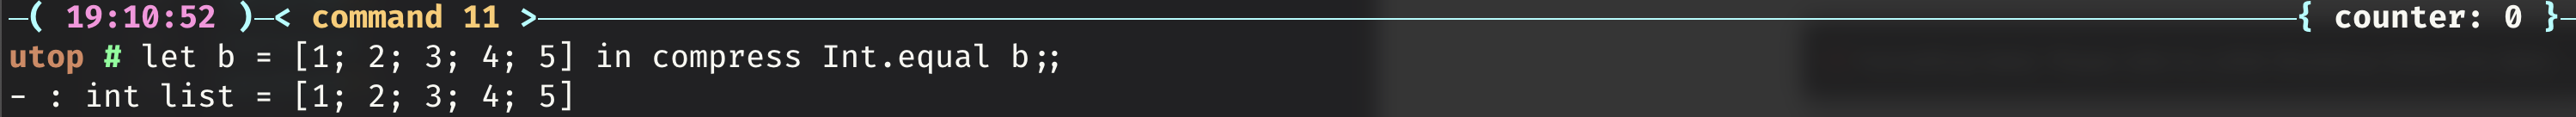
\includegraphics[width=\textwidth]{assets/q2tc3.png}
\end{enumerate}
\newpage
\problem{Merge List}
\solution
\part
\begin{lstlisting}
    let merge (l: 'a option list) : 'a list option =
  let rec merge_helper (acc: 'a list) (l: 'a option list) = 
    match l with
    | [] -> Some (List.rev acc)
    | None::_ -> None
    | Some x::t -> merge_helper (x::acc) t
  in
  merge_helper [] l
\end{lstlisting}
\part
\begin{enumerate}
    \renewcommand{\labelenumi}{\arabic{enumi}.}
    \item \textbf{TestCase 1:} Empty list\newline
    \begin{lstlisting}
        merge [];;
    \end{lstlisting}
    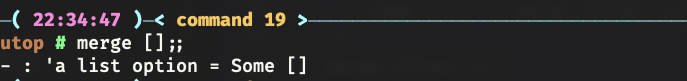
\includegraphics[width=\textwidth]{assets/q3tc1.png}
    \item \textbf{TestCase 2:} List with None\newline
    \begin{lstlisting}
        merge [Some "a"; Some "b"; Some "c"; None; Some "b"];;
    \end{lstlisting}
    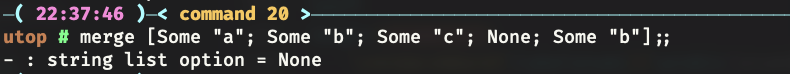
\includegraphics[width=\textwidth]{assets/q3tc2.png}
    \item \textbf{TestCase 3:} List with no None values\newline
    \begin{lstlisting}
        merge [Some 1; Some 3; Some 5];;
    \end{lstlisting}
    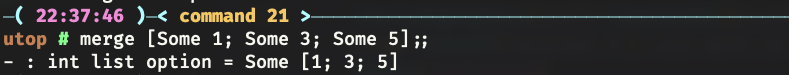
\includegraphics[width=\textwidth]{assets/q3tc3.png}
\end{enumerate}

\problem{Dictionary Functions}
\solution
\part
\begin{lstlisting}
let rec mem (equal: 'k -> 'k -> bool) (k: 'k) (d: ('k * 'v) list) : bool =
  match d with
  | [] -> false
  | (l, j)::t ->
    if equal l k then
      true
    else
      false || (mem equal k t)
\end{lstlisting}

\bigskip

% #TODO: Change these examples.

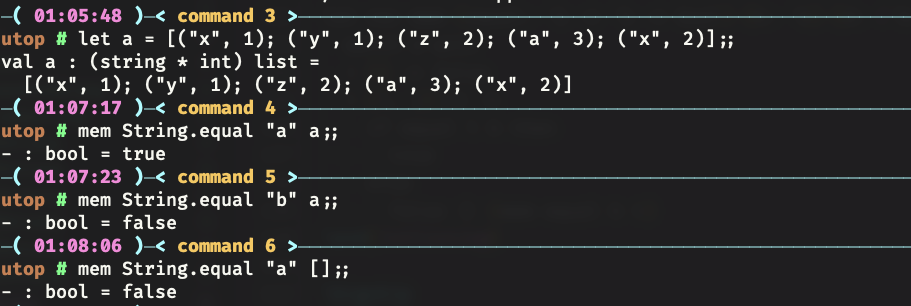
\includegraphics[width=\textwidth]{assets/q4a.png}

\part
\begin{lstlisting}
let rec lookup (equal: 'k -> 'k -> bool) (k: 'k) (d: ('k * 'v) list) : 'v option =
  match d with
  | [] -> None
  | (l, j)::t ->
    if equal l k then
      Some j
    else
      lookup equal k t
\end{lstlisting}
\bigskip

% #TODO: Change these examples.

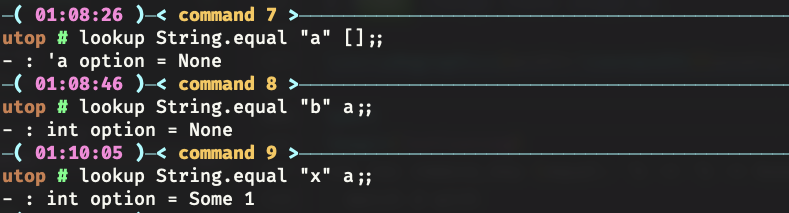
\includegraphics[width=\textwidth]{assets/q4b.png}

\part
\begin{lstlisting}
let rec remove_key (equal: 'k -> 'k -> bool) (k: 'k) (d: ('k * 'v) list) : ('k * 'v) list =
  match d with
  | [] -> []
  | (l, j)::t ->
    if equal l k then
      remove_key equal k t
    else
      (l, j) :: (remove_key equal k t)
\end{lstlisting}

\bigskip

% #TODO: Change these examples.

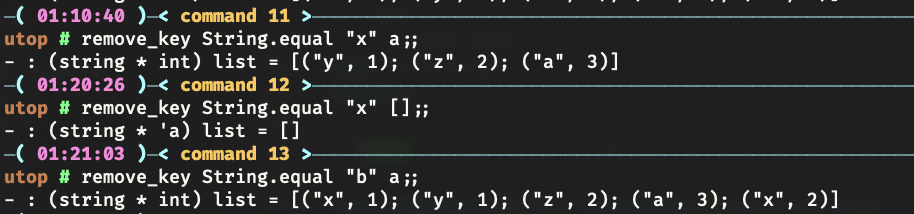
\includegraphics[width=\textwidth]{assets/q4c.png}

\part
\begin{lstlisting}
let rec remove_value (pred: 'v -> bool) (d: ('k * 'v) list) : ('k * 'v) list =
  match d with
  | [] -> []
  | (l, j)::t ->
    if pred j then
      remove_value pred t
    else
      (l, j) :: (remove_value pred t)
\end{lstlisting}

\bigskip

% #TODO: Change these examples.

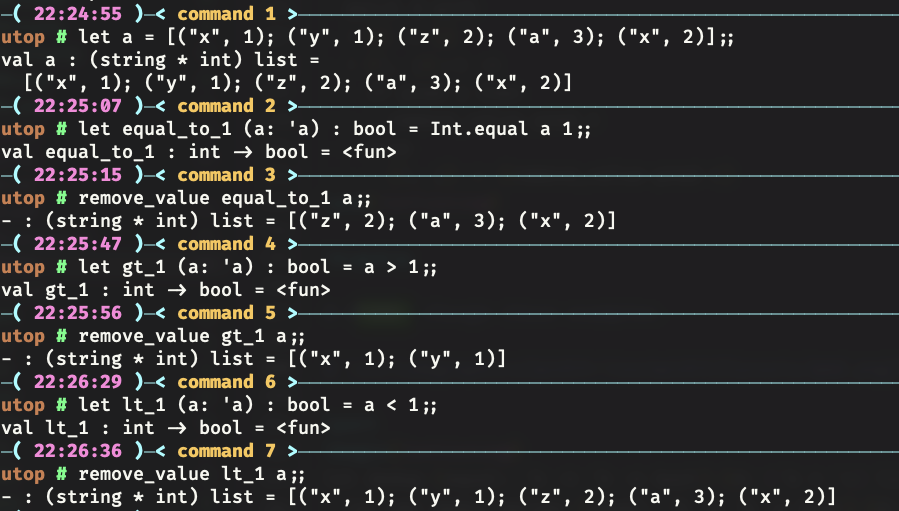
\includegraphics[width=\textwidth]{assets/q4d.png}

\part
\begin{lstlisting}
let dedup (equal: 'k -> 'k -> bool) (d: ('k * 'v) list) : ('k * 'v) list = 
  let rec dedup_helper (equal: 'k -> 'k -> bool) (d: ('k * 'v) list) (acc: ('k * 'v) list) =
    match d with 
    | [] -> (List.rev acc)
    | (l, j)::t -> 
      if (mem equal l acc) then
        dedup_helper equal t acc
      else
        dedup_helper equal t ((l,j)::acc)
  in
  dedup_helper equal d []
\end{lstlisting}

\bigskip

% #TODO: Change these examples.

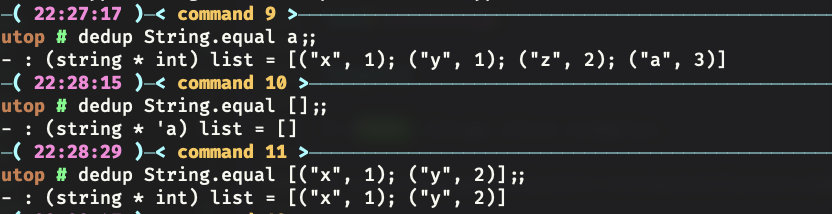
\includegraphics[width=\textwidth]{assets/q4e.png}

\problem{Array operations}
\solution

\part
\begin{lstlisting}
let empty : 'a array = 
  Arr []
\end{lstlisting}

\bigskip

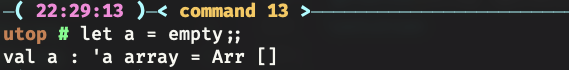
\includegraphics[width=\textwidth]{assets/q5a.png}

\part
\begin{lstlisting}
let select (a: 'a array) (ind: int) : 'a option =
  match a with 
  | Arr [] -> None
  | Arr (x::_ as t) -> lookup Int.equal ind t
\end{lstlisting}

\bigskip

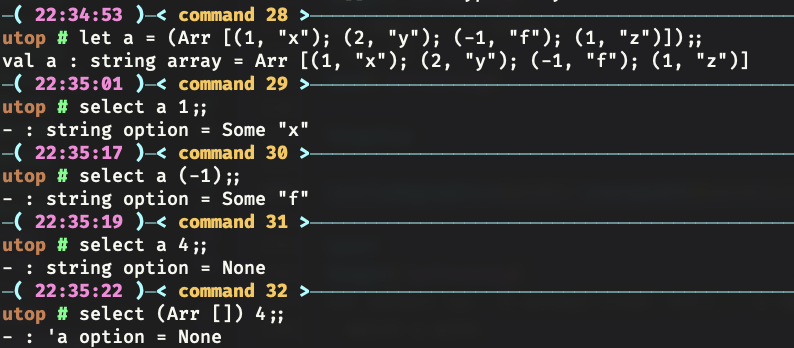
\includegraphics[width=\textwidth]{assets/q5b.png}
\newpage

\part
\begin{lstlisting}
let store (a: 'a array) (ind: int) (value: 'a) : 'a array =
  match a with
  | Arr [] -> Arr [(ind, value)]
  | Arr (x::_ as t) -> Arr (insert ind value t)
\end{lstlisting}

\bigskip

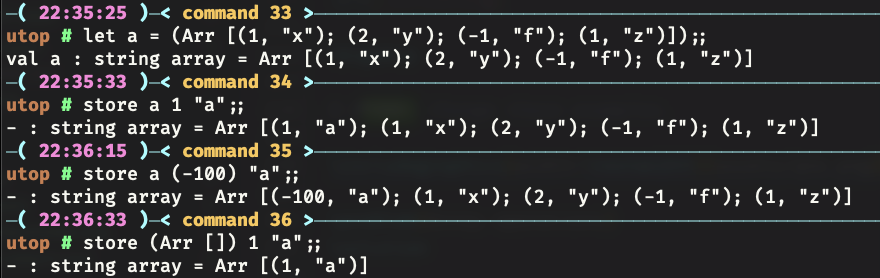
\includegraphics[width=\textwidth]{assets/q5c.png}

\part
\begin{lstlisting}
let of_list (l: 'a list) : 'a array =
  let d = List.mapi (fun i x -> (i, x)) l in
  Arr d
\end{lstlisting}

\bigskip

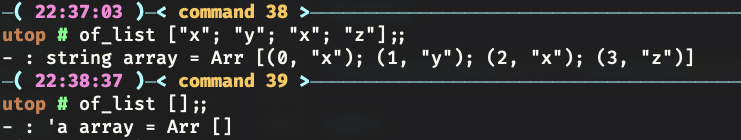
\includegraphics[width=\textwidth]{assets/q5d.png}

\part
\begin{lstlisting}
let unique (a: (int * 'a) list) : (int * 'a) list =
  List.sort_uniq (fun (i, _) (j, _) -> compare i j) a
\end{lstlisting}

\begin{lstlisting}
let to_list (a: 'a array) : 'a list =
  match a with
  | Arr [] -> []
  | Arr l -> List.map snd (unique l)
\end{lstlisting}

\bigskip

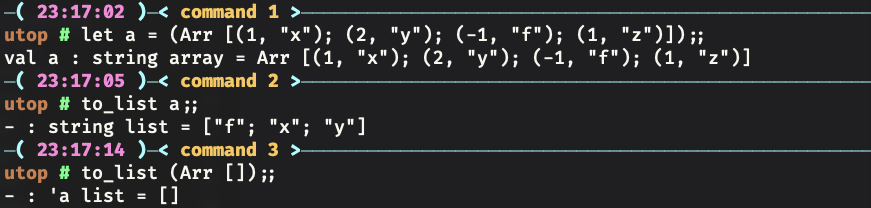
\includegraphics[width=\textwidth]{assets/q5e.png}

\problem{Parse Concrete Syntax to Abstract Syntax Tree}
\solution
\part
\begin{enumerate}
    \renewcommand{\labelenumi}{\arabic{enumi}.}
    \item \textbf{Expression}: $x + y -10$ \newline
        \textbf{AST}: \begin{lstlisting}
           Aop(Sub, Aop(Add, Var "x", Var "y"), Int 10)
        \end{lstlisting}
    \item \textbf{Expression}: $1 - x \geq 3$\newline
        \textbf{AST}: \begin{lstlisting}
            Comp(Geq, Aop(Sub, Int 1, Var "x"), Int 3)
        \end{lstlisting}
    \item \textbf{Expression}: $true$\newline
        \textbf{AST}: $True$
    \item \textbf{Expression}: \begin{lstlisting}
        if z < z { x := 1; } else { y := 2; } 
    \end{lstlisting}
    \textbf{AST}: \begin{lstlisting}
        If(
            Comp(Lt, Var "z", Var "z"), 
            Assign("x", Int 1), 
            Assign("y", Int 2)
        )
    \end{lstlisting}
    \newpage
    \item \textbf{Expression}: \begin{lstlisting}
        x := y;
        y := x; 
        z := x + y;
    \end{lstlisting}
    \textbf{AST}: \begin{lstlisting}
        Seq(
            Assign("x", Var "y"), 
            Seq(
                Assign("y", Var "x"), 
                Assign("z", 
                    Aop(Add, Var "x", Var "y")
                )
            )
        )
    \end{lstlisting}
    \item \textbf{Expression}: \begin{lstlisting}
        while x > 0 {
            if x < 5 {
                x := x + 1;
            } else if x < 10 { 
                x := x + 2;
            } else {
                x := x - 1;
            }
        }
    \end{lstlisting}
    \textbf{AST}: \begin{lstlisting}
        While(
            Comp(Gt, Var "x", Int 0), 
            If(
                Comp(Lt, Var "x", Int 5), 
                Assign("x", Aop(Add, Var "x", Int 1)), 
                If(
                    Comp(Lt, Var "x", Int 10), 
                    Assign("x", Aop(Add, Var "x", Int 2)), 
                    Assign("x", Aop(Sub, Var "x", Int 1))
                )
            )
        )
    \end{lstlisting}
\end{enumerate}
\newpage

\problem{Subsitute Variable}
\solution
\begin{lstlisting}
let rec subst (o: string) (n: string) (exp: aexp) : aexp =
  match exp with
  | Int i -> Int i
  | Var v -> 
    (if String.equal v o then
      Var n
    else
      Var v)
  | Aop (aop, exp1, exp2) -> Aop (aop, (subst o n exp1), (subst o n exp2))
\end{lstlisting}
\bigskip
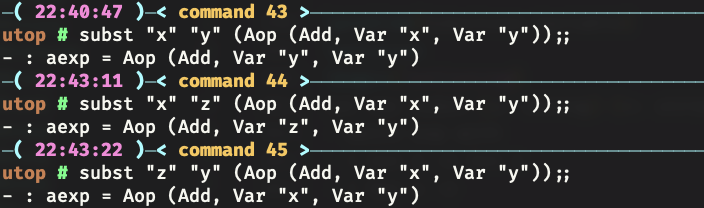
\includegraphics[width=\textwidth]{assets/q7.png}

\problem{Evaluate Abstract Syntax Tree}
\solution
\part
\begin{lstlisting}
let rec lookup (k: 'k) (d: heap) : int option =
  match d with
  | Heap [] -> None
  | Heap ((l, j)::t) ->
    if String.equal l k then
      Some j
    else
      lookup k (Heap t)
\end{lstlisting}

\newpage
\begin{lstlisting}
let insert (k: string) (v: int) (h: heap) : heap = 
  match h with
  | Heap [] -> Heap [(k, v)]
  | Heap t -> Heap ((k, v) :: t)
\end{lstlisting}
\begin{lstlisting}
let calculate_aop (aop: aop) (i1: int) (i2: int) : int =
  match aop with
  | Add -> i1 + i2
  | Sub -> i1 - i2
  | Mul -> i1 * i2

let rec eval_aexp (h: heap) (exp: aexp) : int = 
  match exp with 
  | Int i -> i
  | Var v -> 
    (match (lookup v h) with
    | None -> failwith (Printf.sprintf "No variable %s found" v)
    | Some i -> i)
  | Aop (aop, exp1, exp2) -> (calculate_aop aop (eval_aexp h exp1) (eval_aexp h exp2))
\end{lstlisting}
\bigskip
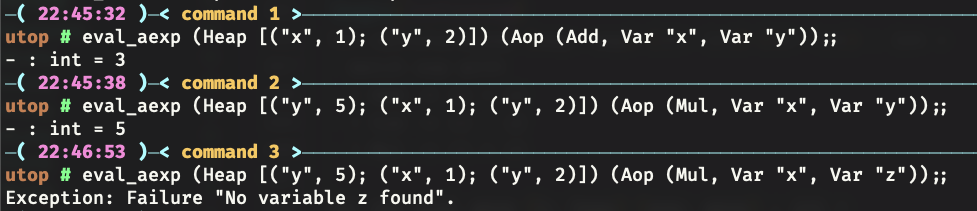
\includegraphics[width=\textwidth]{assets/q8a.png}

\part
\begin{lstlisting}
let calculate_comp (comp: comp) (i1: int) (i2: int) : bool = 
  match comp with 
  | Eq -> (i1 = i2)
  | Geq -> (i1 >= i2)
  | Gt -> (i1 > i2)
  | Lt -> (i1 < i2)
  | Leq -> (i1 <= i2)
  | Neq -> (i1 <> i2)
\end{lstlisting}

\newpage

\begin{lstlisting}
let rec eval_bexp (h: heap) (exp: bexp) : bool = 
  match exp with
  | Bool b -> b
  | Comp (com, exp1, exp2) -> (calculate_comp com (eval_aexp h exp1) (eval_aexp h exp2))
  | Not exp1 ->  (not (eval_bexp h exp1))
  | And (exp1, exp2) -> ((eval_bexp h exp1) && (eval_bexp h exp2))
  | Or (exp1, exp2) -> ((eval_bexp h exp1) || (eval_bexp h exp2))
\end{lstlisting}
\bigskip
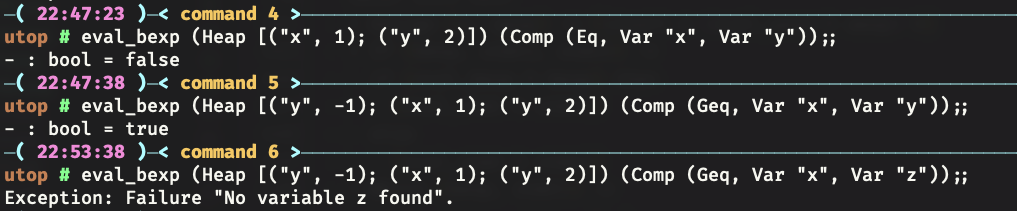
\includegraphics[width=\textwidth]{assets/q8b.png}

\part
\begin{lstlisting}
let rec eval_stmt (h: heap) (stmt: stmt) : heap = 
  match stmt with 
  | Assign (s, aexp) -> (insert s (eval_aexp h aexp) h)
  | If (bexp, stmt1, stmt2) ->
    if (eval_bexp h bexp) then
      (eval_stmt h stmt1)
    else
      (eval_stmt h stmt2)
  | While (bexp, stmt1) -> 
    if (eval_bexp h bexp) then
      (eval_stmt (eval_stmt h stmt1) (While (bexp, stmt1)))
    else
      h
  | Seq (stmt1, stmt2) -> (eval_stmt (eval_stmt h stmt1) stmt2)
\end{lstlisting}
\bigskip
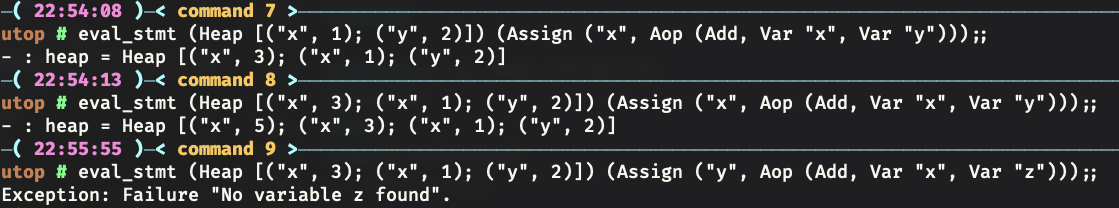
\includegraphics[width=\textwidth]{assets/q8c.png}

\newpage

\problem{Array Read and Write}
\solution
\part
\begin{lstlisting}
x = a[i] * a[j]

Reads:
Path ("a", [Var "i"])
Path ("a", [Var "j"])

AST:
Assign (
  "x",
  Aop (
    Mul,
    Select (Var "a", Var "i"),
    Select (Var "a", Var "j")
  )
)
\end{lstlisting}


\part
\begin{lstlisting}
y = a[a[i]] 

Reads:
Path ("a", [Select (Var "a", Var "i")])

AST:
Assign (
  "y", 
  Select (
    Var "a",
    Select (
      Var "a",
      Var "i"
    )
  )
)
\end{lstlisting}

\part
\begin{lstlisting}
a[x - y] = z

Writes:
Path ("a", [Aop (Sub, Var "x", Var "y")])

AST:
Assign (
  "a",
  Store (
    Var "a",
    Aop (Sub, Var "x", Var "y"),
    Var "z"
  )
)
\end{lstlisting}

\part
\begin{lstlisting}
a[i + j] = a[i] + a[j];

Write:
Path ("a", [Aop (Add, Var "i", Var "j")])

AST:
Assign (
  "a",
  Store (
    Var "a",
    Aop (Add, Var "i", Var "j"),
    Aop (Add, (Select (Var "a", Var "i")), (Select (Var "a", Var "j")))
  )
)
\end{lstlisting}

\part
\begin{lstlisting}
a[a[i]] = y

Writes:
Path ("a", [Select (Var "a", Var "i")])

AST:
Assign (
  "a",
  Store (
    Var "a",
    (Select (Var "a", Var "i")),
    Var "y"
  )
)
\end{lstlisting}

\part
\begin{lstlisting}
a[a[i] + a[j]] = a[a[i] * a[j]]

Reads:
Path ("a", [Aop (Mul, (Select (Var "a", Var "i")), (Select (Var "a", Var "i")))])

Writes:
Path ("a", [Aop (Add, (Select (Var "a", Var "i")), (Select (Var "a", Var "j")))])


AST:
Assign (
  "a",
  Store (
    Var "a",
    Aop (Add, (Select (Var "a", Var "i")), (Select (Var "a", Var "j"))),
    Select (
      Var "a",
      Aop (Mul, (Select (Var "a", Var "i")), (Select (Var "a", Var "j")))
    )
  )
)
\end{lstlisting}

\part
\begin{lstlisting}
a[i][j] = a[j][i]

Reads:
Path ("a", [Var "j"; Var "i"])

Writes:
Path ("a", [Var "i"; Var "j"])

AST:
Assign (
  "a",
  Store (
    Var "a", 
    Var "i", 
    Store (
      (Select (Var "a", Var "i")),
      Var "j",
      (Select (Select (Var "a", Var "j"), Var "i"))
    )
  )
)
\end{lstlisting}

\part
\begin{lstlisting}
a[i][j][k] = a[k][j][i]

Reads:
Path ("a", [Var "k"; Var "j"; Var "i"])

Writes:
Path ("a", [Var "i"; Var "j"; Var "k"])

AST:
Assign (
  "a",
  Store (
    Var "a", 
    Var "i", 
    Store (
      (Select (Var "a", Var "i")),
      Var "j",
      Store(
        (Select (Select (Var "a", Var "i"), Var "j")),
        Var "k",
        (Select (Select (Select (Var "a", Var "k"), Var "j"), Var "i"))
      )
    )
  )
)
\end{lstlisting}

\newpage

\problem{Read and Write from Path}
\solution
\part
\begin{lstlisting}
let rec read_from_path (p: path) : aexp =
  match p with 
  | Path (v, ind_list) -> 
    (match (List.rev ind_list) with
    | [] -> failwith "Empty path"
    | [i] -> (Select (Var v, i))
    | i::t -> Select ((read_from_path (Path (v, (List.rev t))), i))
    )
\end{lstlisting}
\bigskip
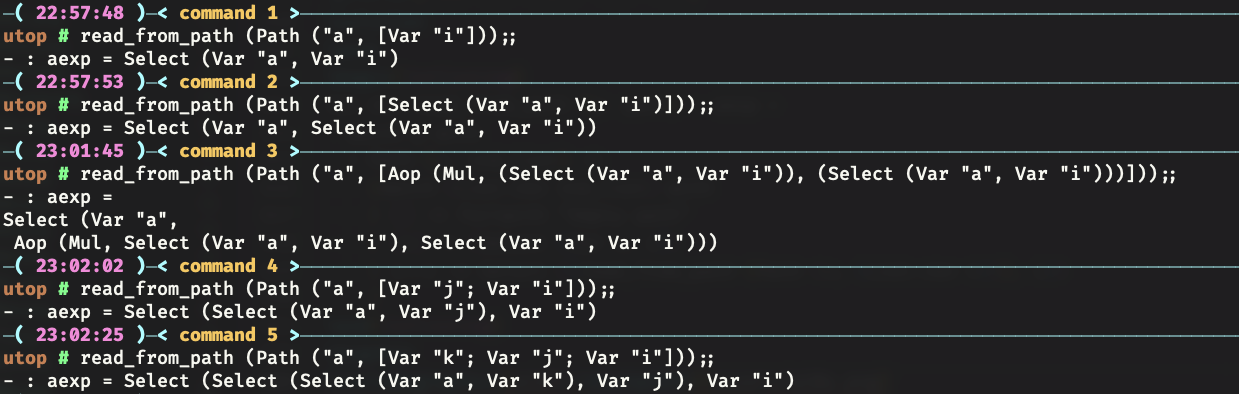
\includegraphics[width=\textwidth]{assets/q10a.png}

\part
\begin{lstlisting}
let write_to_path (p: path) (aexp: aexp) : stmt =
  let rec aux (v: string) (ind_list: aexp list) (aexp: aexp) (read_path: aexp list) : aexp =
    match ind_list with
    | [] -> failwith "Empty Path"
    | [i] -> (Store (Var v, i, aexp))
    | i::t -> (Store ((read_from_path (Path (v, read_path @ [i]))), (aux v t aexp (read_path @ [i])), aexp))
  in
  match p with
  | Path (v, t) -> Assign (v, (aux v t aexp []))
\end{lstlisting}

\end{document}

